% This is samplepaper.tex, a sample chapter demonstrating the
% LLNCS macro package for Springer Computer Science proceedings;
% Version 2.21 of 2022/01/12
%
\documentclass{article}
%
\usepackage[T1]{fontenc}
% T1 fonts will be used to generate the final print and online PDFs,
% so please use T1 fonts in your manuscript whenever possible.
% Other font encondings may result in incorrect characters.
%
\usepackage{graphicx}
%\usepackage{stix}
% Used for displaying a sample figure. If possible, figure files should
% be included in EPS format.
%
% If you use the hyperref package, please uncomment the following two lines
% to display URLs in blue roman font according to Springer's eBook style:
%\usepackage{color}
%\renewcommand\UrlFont{\color{blue}\rmfamily}
%
\usepackage{amsmath}
\usepackage{amsthm}
\usepackage{amsfonts}
\usepackage{tikz}
%\usepackage[font=small,skip=0pt]{caption}
\usepackage{caption}
\usepackage{todonotes}
\captionsetup{font=small,skip=0pt}

\newtheorem{definition}{Definition}
\newtheorem{example}{Example}
\newtheorem{remark}{Remark}
\newtheorem{lemma}{Lemma}

\newcommand{\boundary}{\partial_{k,\ell}}
\newcommand{\imm}{\mathrm{im}}
\newcommand{\vin}{\rotatebox[origin=c]{90}{$\in$}}
\newcommand{\len}{\textsf{len}}
%`` ´´

\newcommand{\giuliaB}[1]{\todo[color=yellow!40]{#1}}
\newcommand{\giuliaBinline}[1]{\todo[inline,color=yellow!40]{#1}}
\newcommand{\giuliaM}[1]{\todo[color=blue!40]{#1}}
\newcommand{\giuliaMinline}[1]{\todo[inline,color=blue!40]{#1}}
\newtheorem{observation}{Observation}
\begin{document}
	%
	\title{On the Relations between Graph Magnitude Homology and Subgraph Counting\thanks{Titolo provvisorio! Altre proposte sono benvenute.}}
	%\title{Relating Graph Magnitude Homology and Subgraph Counting}
	%
	%\titlerunning{Abbreviated paper title}
	% If the paper title is too long for the running head, you can set
	% an abbreviated paper title here
	%
	%\author{First Author\inst{1}\orcidID{0000-1111-2222-3333} \and
	%	Second Author\inst{2,3}\orcidID{1111-2222-3333-4444} \and
	%	Third Author\inst{3}\orcidID{2222--3333-4444-5555}}
	%
	%\authorrunning{F. Author et al.}
	% First names are abbreviated in the running head.
	% If there are more than two authors, 'et al.' is used.
	%
	%\institute{University of Trieste, Trieste, Italy \email{{,,}@units.it} \and
	%}
	%
	\maketitle              % typeset the header of the contribution
	%
	\begin{abstract}
		The abstract should briefly summarize the contents of the paper in
		150--250 words.
		
		%\keywords{First keyword  \and Second keyword \and Another keyword.}
	\end{abstract}
	
	%
	%
	%
	%1) scrivere intuizione prima di definizione
	%2) rendere più operative le definizioni
	%
	
	\section{Introduction (DA SISTEMARE)}
	
	Graphs are used in a variety of sciences to model and to analyze complex relationships. 
	In this framework, the search for interesting and relevant substructures is a standard procedure, and the detection of cliques and clique-like subgraphs is a fundamental tool in graph analysis.
	Such substructures have been applied in many different situations including community detection in social networks \cite{kumar1999trawling}, \cite{sozio2010community}, identification of real-time stories in the news \cite{angel2014dense} and graph visualization \cite{zhang2012extracting}, \cite{zhao2012large}.
	In practice, due to noise in data, one is also interested in large ``near-cliques''. 
	While this is not a standard term, applications involve cliques that are missing a small sparse subgraph.
	For example, incomplete cliques have been used to predict missing pairwise interactions \cite{zhang2012extracting} and for identifying functional groups \cite{han2007identifying} in a protein interaction network. 
	Also, they were exploited for community detection \cite{zhu2020community} and for detecting test collusion \cite{belov2021graph}.
	Recent works have used the fraction of near-cliques to k-cliques to define higher order variants of clustering coefficients \cite{yin2017local}.
	
	In the present work, in order to quantitatively characterize these structures, we employ magnitude homology, a tool that comes from the field of algebraic topology.
	Magnitude is an isometric invariant of metric spaces, so-named for its web of connections to ``size-like'' quantities of significance in various corners of mathematics.
	Defined and first studied by Leinster \cite{leinster2013magnitude}, it is a special case of a general theory of magnitude of an enriched category, and has found applications in areas like biodiversity (e.g., Leinster and Cobbold \cite{leinster2012measuring}).
	As a finite graph naturally gives rise to a finite metric space, it is possible to associate magnitude with it.
	Magnitude homology has been invented by Hepworth and Willerton \cite{hepworth2015categorifying} as an enrichment of the magnitude of a graph which is equipped with a graph metric.
	The magnitude homology of graphs has been well studied in recent years and has proven to be a rich invariant \cite{hepworth2015categorifying,gu2018graph,sazdanovic2021torsion,hepworth2022magnitude,kaneta2021magnitude}.
	Also, several theoretical tools for computing the magnitude homology of a graph have been studied so far. 
	For example, Hepworth and Willerton proved in \cite{hepworth2015categorifying} a Mayer-Vietoris type exact sequence and a Kunneth type formula, %\giuliaM{@GiuliaB, ho aggiunto la citazione. Non so se si possono definire tool algoritmiche.. la prima è un po' più spendibile in pratica (mette in relazione $MH(G \cap H)$ con $MH(G \cup H)$ e $MH(G) \oplus MH(H)$), la seconda è interessante dal punto di vista teorico ma dovrei pensare a come calarla in uno contesto più applicato}
	%\giuliaB{Grazie! Probabilmente per questo articolo non serve che ci concentriamo su quello, comunque! Volevo solo essere sicura di scrivere cose corrette nel progetto :)}
	and Gu \cite{gu2018graph} uses algebraic Morse theory for computation for some graphs. 
	Although, in general, computation of magnitude homology remains a difficult problem.
	
	\textbf{TBC}
	
	In this work,...
	
	The paper is organized as follows,...
	
	\section{Background}
	
	An undirected graph is a pair $G=(V,E)$ where $V$ is a set of vertices and $E$ is a set of edges (unordered pairs of vertices). A \emph{trail} in $G$ is a sequence of vertices $x_1,x_2,\ldots,x_n$ such that there is an edge $\{x_i,x_{i+1}\}$ for all $0\leq i<n$; a \emph{path} is a trail with no repeated vertices; a \emph{cycle} is a closed path.
	For the purposes of defining magnitude homology, we assume all graphs to have no self-loops and no multi-edges \cite{leinster2019magnitude}.
	We define the distance $d:V \times V \to [0,\infty]$ between two vertices $u,v \in V$  as the length of the shortest path from $u$ to $v$, with $d(u,v) = \infty$ if $u$ and $v$ lie in different connected components.
	%
	%We recall Hepworth and Willerton's construction \cite{hepworth2015categorifying} of the magnitude homology groups of a graph.
	
	A $k$-trail in a graph $G$ is a $k$-tuple $\overline{x}^k=(x_1,\dots,x_k)$ 
	of \emph{required vertices}  with $x_i \neq x_{i+1}$ and $d(x_i,x_{i+1})<\infty$ for every $1 \leq i \leq k-1$.
	The length of a $k$-trail $\overline{x}^k$ is defined as the minimum length of a trail that visits $x_1,\ldots,x_k$ in this order (i.e., whose visited vertices form a supersequence of the required vertices): namely, 
	\(
	\len(\overline{x}^k) = d(x_1,x_2)+\cdots + d(x_{k-1},x_k).
	\) 
	
	A triangle in $G$ is a cycle on 3 distinct vertices; a \emph{chordless} or \emph{induced} square is a cycle connecting four distinct vertices $x_1,x_2,x_3,x_4$ such that there are no edges between them except the edges of the cycle: in other words, $\{x_1,x_3\}\notin E$ and $\{x_2,x_4\}\notin E$. 
	A $k$-clique is a subset of $k$ distinct vertices s.t. every two distinct vertices n the clique are connected by an edge.
	
	A \emph{free abelian group} is an abelian group (a set of elements with a sum operation) that has a basis, that is, a finite subset of its elements s.\@t.\ all the other elements can be expressed as an integer combination of the elements of the basis. We will denote by $\langle B\rangle$ the free abelian group \emph{generated} by the basis $B$. The \emph{rank} of a group is the number of elements of a basis.%the elements of a free abelian group may be thought of as signed multisets containing finitely many elements of the basis, with the multiplicity of an element in the multiset equal to its coefficient in the formal sum.
	%\begin{example}
	%   The integers $\mathbb{Z}$ form a free abelian group with basis $\{1\}$. Also, the polynomials in one variable $x$ with integer coefficients form a free abelian group with the powers of $x$ as basis.  
	%\end{example}
	
	The $(k,\ell)$-\emph{magnitude group} of a graph, denoted by $M_{k}^{\ell}$, is the free abelian group generated by all the $k$-trails of length $\ell$ in the graph\footnote{Formally, $M_{k}^{\ell}$ is called the $(k,\ell)$-magnitude chain~\cite{hepworth2015categorifying}. 
		See definition~\ref{def:magchain} in Appendix~\ref{app:algebra}.}.
	Assuming that the vertices of the graph are in a one-to-one correspondence with the integers in $[1,|V|]$, we can lexicographically order the $k$-tuples: we denote by $M_{k}^{\ell}[j]$ the $j$-th lexicographically smallest element of $M_{k}^{\ell}$. 
	We denote by $\overline{x}_{\hat{\imath}}^k$ the $(k-1)$-tuple $(x_1,\ldots,x_{i-1},x_{i+1},\ldots,x_k)$ obtained removing the $i$-th required vertex from $\overline{x}^k$.
	
	\begin{definition}
		\label{def:dif_matrix}
		Consider $M_{k}^{\ell}$ and $M_{k-1}^{\ell}$. The \emph{differential matrix} $\Delta_k^\ell=\{\delta_{r,c}\}$ is the matrix whose $c$-th column corresponds to $M_{k}^{\ell}[c]$, whose $r$-th row corresponds to $M_{k-1}^{\ell}[r]$, and with 
		%
		%\partial_k: M_{k}^{\ell} \to M_{k-1}^{\ell}
		%
		\[\delta_{r,c}=\begin{cases}
			(-1)^{i} &\text{ if } M_{k}^{\ell}[c]=\overline{x}^k \land M_{k-1}^{\ell}[r]=\overline{x}_{\hat{\imath}}^k, \\
			0 &\text{ otherwise.}\\
		\end{cases}
		\]
	\end{definition}
	%
	Note that each nonzero entry of $\Delta_k^\ell$ corresponds to some $k$-trail of length $\ell$ whose length does not decrease when some required vertex $x_i$ is removed\footnote{Formally, $\Delta_k^\ell$ is the matrix representation of a differential map between free abelian groups. 
		See Definition~\ref{differential} in Appendix~\ref{app:algebra}.}, implying that there is no shortcut that connects $x_{i-1}$ and $x_{i+1}$ without using $x_i$. 
	This provides some information on the structure of $G$, in particular on the occurrences of specific subgraphs, as we show in Section~\ref{sec:subgraphs}.
	
	Clearly, we can define a sequence of differential matrices $\Delta_k^\ell, \Delta_{k-1}^\ell, \Delta_{k-2}^\ell\ldots$ that relate the elements of the magnitude groups for a fixed $\ell$ and decreasing $k$. 
	This sequence has an analogous algebraic definition, given in Appendix~\ref{app:algebra}, that motivates the following definition.
	
	\begin{definition}
		\label{def:Hset}
		The $(k,\ell)$-magnitude homology group of a graph $G$ is the group \giuliaBinline{@GiuliaM, con questa definizione però il ker è generato solo dalle colonne nulle, è giusto?}
		\giuliaMinline{No così dovremmo beccare anche le combinazioni, perché $M_k^{\ell}$ è un gruppo libero e quindi contiene anche le somme formali. Quindi (prendendo l'esempio sotto) abbiamo che $(0,1,2)-(0,3,2) \in M_k^{\ell}$ e $\len((0,\hat{1},2)-(0,\hat{3},2))=0$, per cui $(0,1,2)-(0,3,2)$ sta nel ker.}
		\giuliaBinline{Ma $\overline{x}^k$ è definita come tupla che determina un $k$-trail, non come generico elemento del gruppo...e la lunghezza di una somma formale non è definita (non avrebbe neanche senso, non corrispondendo a un percorso). secondo me quindi dobbiamo formularlo diversamente, ma possiamo pensarci dopo.}
		\giuliaMinline{Forse possiamo definire il kernel direttamente come kernel della matrice, visto che il nostro operatore è proprio costruito così. Perché quello che si fa di solito è definire l'operatore differenziale e poi dire ``siccome è lineare ha una matrice associata e calcoliamo rango e dimensione del nucleo della matrice associata". Qua non dovremmo neanche fare questo passaggio}
		\giuliaBinline{concordo pienamente. Poi sotto mettiamo l'osservazione sulle colonne nulle e bon}
		\[
		H_k^\ell = \ker(\Delta_k^\ell)\setminus\imm(\Delta_{k+1}^\ell), \text{where}~\ker(\Delta_k^\ell)=\langle\overline{x}^k \in M_k^\ell \mid \len(\overline{x}_{\hat{\imath}}^k)<\ell\ \forall~ i\rangle~\text{and}
		\]
		\[
		\imm(\Delta_k^\ell) =\langle\overline{x}^{k-1} \in M_{k-1}^\ell \mid \exists i\in[1,k-1] \text{and}~ \overline{x}^k\in M_k^\ell~\text{s.t.}~\overline{x}^{k-1}=\overline{x}_{\hat{\imath}}^k\rangle.
		\]
	\end{definition}
	In other words, the $(k,\ell)$-magnitude homology group is generated by the $k$-trails of length $\ell$ that cannot be obtained by removing a required vertex from some $(k+1)$-trail of length $\ell$, and whose length decreases if any of their required vertices are removed.
	
	\begin{example}
		\label{ex:toyexample_standard_def}
		Consider the following graph $G$, for which we want to compute $H_3^2$.
		
		\begin{center}
			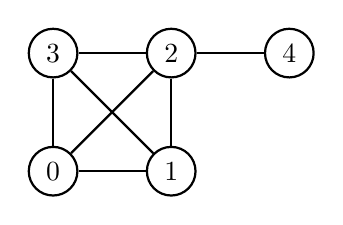
\begin{tikzpicture}[node distance={15mm}, thick, main/.style = {draw, circle}]
				\node[main] (0) {$0$}; 
				\node[main] (1) [right of=0] {$1$}; 
				\node[main] (2) [above of=1] {$2$}; 
				\node[main] (3) [above of=0] {$3$}; 
				\node[main] (4) [right of=2] {$4$};
				\draw (0) -- (1);
				\draw (0) -- (2);
				\draw (0) -- (3);
				\draw (1) -- (2);
				\draw (1) -- (3);
				\draw (2) -- (3);
				\draw (2) -- (4);
			\end{tikzpicture} 
		\end{center}
		
		From Definition \ref{def:Hset} we need to compute the difference set between the kernel of $\Delta_3^2$ and the image of $\Delta_4^2$, so we are concerned with the three magnitude sets $M_{2}^{2}$, $M_{3}^{2}$, $M_{4}^{2}$.
		By definition, $M_{2}^{2}$ consists of the $2$-trails of length $2$, that is, $M_{2}^{2}=\{(0, 4), (1, 4), (3, 4), (4, 0), (4, 1), (4, 3)\}$.
		Similarly, $M_{3}^{2}$ consists of the $3$-trails of length $2$, i.e., it is the following set of $44$ elements: 
		%$\{(i,j,i)\mid i,j\in[0,3],i\neq j \}\cup \{(i,j,i)\mid i,j\in\{2,4\},i\neq j\} \cup \{(i,j,k)\mid i,j,k\in[0,3],i\neq j\neq k\}\cup \{(i,j,4)\mid i,j\in[1,3],i\neq j\}\cup\{(4,i,j)\mid i,j\in[1,3],i\neq j\} \cup (0, 2, 4) \cup (4, 2, 0)$.
		$\{(h,i,j)\mid h,i,j\in[0,3],h\neq i,i\neq j\}\cup \{(i,2,4)\mid i\neq 2\}\cup\{(4,2,i)\mid i\neq 2\}$.
		Finally, $M_{4}^{2}$ consists of the $4$-trails of length $2$, and since any trail connecting 4 vertices has length at least 3, we have $M_{4}^{2}=\emptyset$.
		
		We see from Figure~\ref{fig:delta22} that $\Delta_3^2$ has no linear dependent columns, thus $\ker(\Delta_3^2)$ is generated by the elements of $M_{3}^{2}$ whose length diminishes when the middle vertex is removed (corresponding to the null coulmns): $$\ker(\Delta_3^2)=M_{3}^{2}\setminus \{(0, 2, 4), (1, 2, 4), (3, 2, 4), (4, 2, 0), (4, 2, 1), (4, 2, 3)\}.$$
		Since $M_{4}^{2}=\emptyset$, we have that $\imm(\Delta_4^2)=\emptyset$ and thus the 3-magnitude homology group of $G$ coincides with the 38 elements in the kernel of $\Delta_3^2$.
	\end{example}
	\begin{figure}
		\centering
		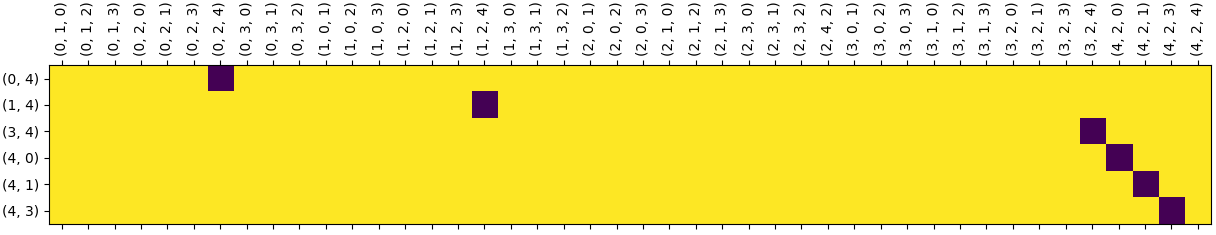
\includegraphics[width=\textwidth]{images/kernel_toy_example.png}
		\caption{Matrix $\Delta_3^2$. The $+1$ entries are in purple, while the $0$ entries are in yellow.}\label{fig:delta22}
	\end{figure}
	
	In the following we will focus on the matrix $R=\{r_{\ell,k}\}$ \giuliaB{Questo paragrafo può essere migliorato.} of the ranks of the homology groups $H_k^\ell$, that is, $r_{\ell,k}=|H_k^\ell|$.
	We call $R$ the \emph{rank matrix} of $G$. 
	\begin{observation}
		\label{LowerTriangRem}
		%$R$ is lower triangular, that is, $r_{k,\ell}\neq 0$ implies that $\ell\geq k-1$.
		Note that $R$ is such that $r_{k,\ell}=0$ for all $k,\ell$ such that $\ell>k-1$.
		This is because if $H_{k}^{\ell}\neq \langle 0 \rangle$ then $M_{k}^{\ell}\neq \langle 0 \rangle$, and so there is at least a tuple $(x_1,\dots,x_k)$ satisfying $\len(x_1,\dots,x_k)=d(x_1,x_2)+\cdots+d(x_{k-1},x_k) = \ell$.
		Now, since consecutive vertices are distinct by construction, $d(x_i,x_{i+1})$ is at least $1$ for every $1\leq i\leq k-1$, which means $k$ can be at most $\ell+1$.
		
		\begin{table}
			\centering
			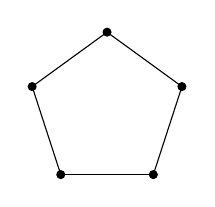
\begin{tikzpicture}[scale=0.5]
				\foreach \x in {0,72,...,288}
				\draw (\x+90:2cm) -- (\x+72+90:2cm);
				\foreach \x in {0,72,...,288}
				\draw [fill](\x+90:2cm) circle (0.1cm);
			\end{tikzpicture}
			\quad
			\begin{tabular}{rr|rrrrrr}
				&&&&$k$&\\
				&&1&2&3&4&5\\ 
				\hline                                                               
				& 0 &5\\
				& 1 & &10\\                                          
				& 2 & & &10\\                                          
				$l$& 3 & & &10 &10\\                                          
				& 4 & & &   &30 &10\\                                         
				& 5 & & &   &   &50 \\           
			\end{tabular}
			%\end{center}
			\caption{Ranks of $H_k^{\ell}(C_5)$ computed using Python \cite{code2022magnitude}}
			\label{table:TableC5}
		\end{table}
	\end{observation}
	
	In what follows we refer to the set of the ranks of the $H_k^{k-1}$ homology groups (that is, the top non-zero diagonal in the rank matrix) as \emph{first diagonal}.
	Accordingly, the \emph{$n$-th diagonal} will identify the ranks of the $H_k^{k-n}$ homology groups.
	\\
	
	It is proven in \cite{hepworth2015categorifying} (Proposition 9) that given a graph $G$, if we indicate by $V$ the set of vertices and by $2E$ the set of oriented edges, then $H_1^0(G)$ is the free abelian group on $V$ and $H_2^1(G)$ is the free abelian group on $2E$.
	
	This provides us with an interpretation of the first two diagonals but leaves the question about the meaning of other magnitude homology groups open.
	
	\section{Interpretation of magnitude homology}\label{sec:subgraphs}
	
	In this section, we provide an interpretation for some of the magnitude homology groups corresponding to elements on the first and second diagonals of the rank matrix.
	To this aim, we introduce a slightly different notion of magnitude group, which avoids considering as generators the $k$-trails that carry redundant information on the structure of the graph. 
	
	First, notice that the $k$-tuples $(x_1,\dots,x_k)$ and $(x_k,\dots,x_1)$ represent exactly the same subset of vertices and edges of $G$, and thus one of the two is redundant. Without loss of generality, we define the lexicographically smallest of the two as the \emph{representative} of the two possible orientations of the $k$-trail they represent, and we will disregard the other.
	
	The trails with some repeated required vertices are redundant too. An example can be seen on the magnitude group $M_{3}^{2}$ for the graph of Example \ref{ex:toyexample_standard_def}:
	the 3-trail $(0, 1, 0)$ consists in traversing the edge $(0, 1)$ twice, thus it does not provide any additional information about the structure of the graph with respect to the 2-trail $(0,1)$. 
	
	We thus define the \emph{normalized} magnitude group as the subgroup of $M_{k}^{\ell}$ generated by the representative $k$-trails of length $\ell$ with no repeated required vertices.
	
	\begin{definition}\label{def:normalised}
		The normalized $(k,\ell)$-magnitude group $\widehat{M}_{k}^{\ell}$ of a graph $G$ is the free abelian group generated by the representative $k$-trails $\overline{x}^k=(x_1,\dots,x_k)$ of length $\ell$ and such that $x_i \neq x_j$ for every $i\neq j$.
	\end{definition}
	
	\begin{observation}\label{obs:representatives}
		If $\overline{x}^k$ is a generator of a normalized magnitude group, then $\overline{x}^k_{\hat{\imath}}$ is a representative $(k-1)$-trail for all $1<i<k$. 
	\end{observation}
	\begin{proof}
		It follows immediately from the fact that all the vertices in a generator $\overline{x}^k=(x_1,\ldots,x_k)$ of a normalized magnitude group are distinct, and since by definition $\overline{x}^k$ is a representative $k$-trail it holds that $x_1<x_k$, which remains true removing any intermediate required vertex.\qed
	\end{proof}
	
	The differential matrix $\widehat{\Delta}_k^\ell$ and the homology group $\widehat{H}_k^\ell$ for the normalized magnitude groups are defined entirely analogously to the magnitude groups.
	
	\begin{example}\label{ex:normalised_groups}
		Consider the same graph $G$ as in Example \ref{ex:toyexample_standard_def}.
		By Definition \ref{def:normalised}, the normalized magnitude group $\widehat{M}_{3}^{2}$ is generated by the subset of generators of $M_3^2$ consisting of the following $15$ elements (see also Figure~\ref{fig:normalized_delta22}): 
		$$\{(h,i,j)\mid i,j\in[0,3], h\in[0,j),h\neq i\neq j\}\cup \{(i,2,4)\mid i\in[0,3]\}.$$
	\end{example}
	
	\begin{remark}
		\label{NMHsubgroup}
		We point out that all definitions and properties regarding magnitude homology proved in \cite{hepworth2015categorifying} and \cite{leinster2021magnitude} are still valid for the normalized magnitude homology groups.
		This is because, by construction, $\widehat{M}_k^{\ell}$ is a subgroup of $M_k^{\ell}$ (as it is generated by a subset of its generators), and since the definition of the differential matrix is unchanged it follows that the normalized magnitude homology group $\widehat{H}_k^{\ell}$ is a subgroup of  $H_k^{\ell}$ for every $k,\ell\geq 0$.
		
		In particular, with this new definition, $\widehat{H}_1^{0}$ and $\widehat{H}_2^1$ are still counting the number of vertices and edges in a graph respectively, because the generators of the groups $M_1^0$ and $M_2^1$ already satisfy the condition of not revisiting vertices.
	\end{remark}
	
	\subsection{First diagonal: counting triangles and squares}
	\label{FirstDiagonal}
	In this section, we focus on the groups $\widehat{H}_k^{k-1}$.
	As already noticed in Observation~\ref{LowerTriangRem}, the image of $\widehat{\Delta}_{k+1}^{k-1}$ is the zero group $\langle 0 \rangle$ for all values of $k$, and thus the normalized homology group $\widehat{H}_k^{k-1}$ coincides, by Definition~\ref{def:Hset}, with $\ker(\widehat{\Delta}_k^{k-1})$.
	
	Let us start by considering the normalized homology group  $\widehat{H}_3^2=\ker(\widehat{\Delta}_3^2)$ of an undirected graph $G$, and consider the differential matrix $\widehat{\Delta}_3^2$. Recall that the columns of $\widehat{\Delta}_3^2$ correspond to the generators of $\widehat{H}_3^2$, i.e., the representative 3-trails of length 2 in $G$ with no repeated required vertices. We have the following simple lemma.
	
	\begin{lemma}\label{lem:triangles}
		Let Z be the number of null columns of $\widehat{\Delta}_3^2$. The number of triangles occurring in $G$ is $\frac{Z}{3}$.
	\end{lemma}
	
	\begin{proof}
		Consider a representative $3$-trail $\overline{x}=(x_1,x_2,x_3)$ of length 2 and suppose w.\@l.\@o.\@g.\ that $x_1< x_2< x_3$. Since $\overline{x}$ has length 2, $\{x_1,x_2\}$ and $\{x_2,x_3\}$ are edges of $G$. 
		By Definition~\ref{def:dif_matrix}, $\overline{x}$ corresponds to a zero column of $\widehat{\Delta}_3^2$ if and only if the shortest path between $x_1$ and $x_3$ has length smaller than $2$, that is, if removing the required vertex $x_2$ we obtain a 2-trail of length 1. 
		This implies that there exists and edge $\{x_1,x_3\}$ and thus a triangle with vertices $x_1,x_2,x_3$.
		
		It is immediate to see that $\overline{x}'=(x_1,x_3,x_2)$ and $\overline{x}''=(x_2,x_1,x_3)$ are the only other representative 3-trails whose vertices are a permutation of $x_1,x_2,x_3$, that $\overline{x}'$ and $\overline{x}''$ correspond to null columns and thus that they identify the same triangle in $G$ as $\overline{x}$.
	\end{proof}
	
	%A direct consequence of Lemma~\ref{lem:triangles} is that the number of triangles occurring in $G$ is given by the number of null columns of $\widehat{\Delta}_3^2$ divided by $3$, i.e., by the cardinality of the automorphisms group of the triangle $D_3$ (the number of permutations of its vertices) restricted to the three representative.\giuliaM{@GiuliaB ho dovuto così perché purtroppo non ci viene un sottogruppo di $D_3$. Va bene o è troppo vago?}
	
	%\giuliaB{Ho cambiato direttamente l'enunciato del lemma e la dimostrazione, come ti pare?}
	%\giuliaM{Top :)}
	
	\begin{example}\label{ex:triangles}
		Consider the same graph $G$ as in Example \ref{ex:toyexample_standard_def}.
		We want to compute $\widehat{H}_3^2$.
		The generators of $\widehat{M}_3^2$ are shown in Example \ref{ex:normalised_groups};
		further, $\widehat{M}_2^2$ is generated by the $2$-trails $(0,4)$, $(1,4)$ and $(3,4)$ and the differential matrix $\widehat{\Delta}_3^2$ (shown in Figure~\ref{fig:normalized_delta22}) is the submatrix of the one displayed in Figure \ref{fig:delta22} whose columns and rows correspond to the generators of $\widehat{M}_3^2$ and $\widehat{M}_2^2$, respectively.
		We see that $\widehat{\Delta}_3^2$ has 12 null columns, corresponding to the four triangles of vertices $\{0, 1, 3\}$, $\{0, 1, 2\}$, $\{0, 2, 3\}$ and $\{1, 2, 3\}$, respectively.
		\begin{figure}
			\centering
			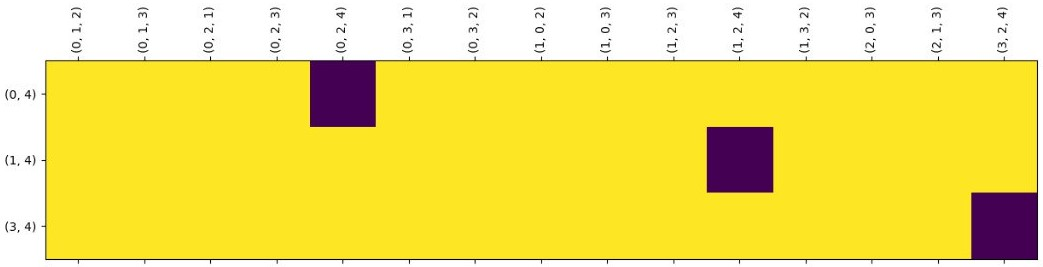
\includegraphics[width=\textwidth]{images/normalized_matrix_example.jpg}
			\caption{Matrix $\widehat{\Delta}_3^2$. The $+1$ entries are in purple, while the $0$ entries are in yellow.}\label{fig:normalized_delta22}
		\end{figure}
	\end{example}
	
	Let us now focus on the linearly dependent nonzero columns of $\widehat{\Delta}_3^2$. 
	We start by observing the following.
	
	\begin{observation}\label{obs:repeated_columns}
		The linearly dependent nonzero columns of $\widehat{\Delta}_3^2$ are all and only the columns that are repeated at least twice.
	\end{observation}
	\begin{proof}
		By Definition~\ref{def:dif_matrix}, an entry of $\widehat{\Delta}_3^2$ is equal to 1 if and only if $\len(x_1,x_2,x_3)=\len(x_1,x_3)=2$.
		Thus in the column corresponding to $(x_1,x_2,x_3)$ the only entry that can possibly be 1 is the one at the row corresponding to $(x_1,x_3)$.
		Therefore, two nonzero columns can only be linearly dependent if they are equal, and this can happen only if they correspond to two triplets $(x_1,x_2,x_3),(x_1,x'_2,x_3)$ that share the same first and last vertex.
		This implies that the subset of linearly dependent columns of $\widehat{\Delta}_3^2$ coincides with the columns that are repeated at least twice.\qed
	\end{proof}
	
	The following lemma provides a first (rough) upper bound on the number of chordless squares in $G$.
	
	\begin{lemma}\label{lem:squares}
		Let $N$ be the number of linearly dependent nonzero columns of $\widehat{\Delta}_3^2$. The number of chordless squares in $G$ is upper bounded by $\frac{(N-1)N}{2}$.
	\end{lemma}
	\begin{proof}
		Notice that a necessary (yet not sufficient) condition for the presence of a chordless square of vertices $w,x,y,z$  in $G$ is that there exist two generators of $\widehat{M}_3^2$, $(x,y,z)$ and $(x,w,z)$, such that there is no edge linking $x$ and $z$. In particular, the absence of the edge $\{x,z\}$ implies that the length of $(x,y,z)$ and $(x,w,z)$ does not decrease removing the respective intermediate required vertices, and thus the corresponding columns of $\widehat{\Delta}_3^2$ both have a 1 at the row corresponding to $(x,z)$. Thus two equal nonzero columns imply the presence of a square in $G$ which is not a clique (yet there could be the edge $\{w,y\}$ that makes the square not chordless). 
		
		Suppose now there is a third generator with the same endpoints $(x,v,z)$. Since $\{x,z\}\notin E$, the column of $\widehat{\Delta}_3^2$ corresponding to $(x,v,z)$ has a 1 at the row corresponding to $(x,z)$ too. It is easy to see that these three generators imply the presence of 3 squares that are not cliques: one having vertices $x,w,z,y$, another with vertices $x,w,v,y$ and a last one with vertices $v,y,z,w$. Three linearly dependent columns thus imply $\frac{(3-1)3}{2}=3$ squares occurring in $G$.
		
		Let us now generalize this formula to $M$ equal columns and prove by induction that they imply the presence of $\frac{(M-1)M}{2}$ squares that are not cliques. We already verified that the formula holds for the base case $M=2$ and for $M=3$. Let us assume it holds for $M-1$ equal columns, which thus identify $\frac{(M-2)(M-1)}{2}$ non-cliques squares, and suppose there is an $M$-th equal column. The $3$-trail corresponding to such column gives rise to a new distinct square with each one of the other $M-1$ $3$-trails with the same endpoints, thus giving a total of $\frac{(M-2)(M-1)}{2} + (M-1)= \frac{(M-1)M}{2}$ non-cliques squares.
		
		It is immediate to see that if the generators corresponding to all the $N$ linearly dependent nonzero columns do not have all the same endpoints, the number of non-cliques squares in $G$ is strictly less than $\frac{(N-1)N}{2}$; and since the chordless squares are included in the set of non-cliques squares, this quantity trivially bounds their occurrences in $G$.\qed
	\end{proof}
	
	Notice that the bound provided by Lemma~\ref{lem:squares} is rather coarse. In fact, it actually bounds the total number of 4-cycles that are not 4-cliques in the graph, which also include the 4-cycles with one crossing edge (see Figure...........\giuliaB{Possiamo mettere un piccolo esempio solo se abbiamo spazio alla fine: @GiuliaM, se ti va comunque potresti fare una figurina in cui ci sono un tot di quadrati inscatolati e quello più all'interno ha un lato orizzontale, poi se non c'è posto la piazziamo in appendice.})
	A closer look at the linearly dependent columns allows us to provide a stricter bound, given in Lemma~\ref{lem:squares_stricter}, which again bounds the total number of 4-cycles that are no cliques in the graph.
	
	In order to compute the exact number of \emph{chordless} squares, not only do we need to consider the linearly dependent columns themselves but also the generators they correspond to: we give this result in Lemma~\ref{lem:chordless_squares}.
	
	\begin{lemma}\label{lem:squares_stricter}
		Let $D$ be the collection of linearly dependent nonzero columns of $\widehat{\Delta}_3^2$, let $c_1,\ldots,c_u$ be the largest subset of columns in $D$ s.t. $c_i\neq c_j~\forall i,j\in[1,u]$ and let $n_i$ be the number of times a column $c_i$ occurs in $D$. The number of chordless squares in $G$ is upper bounded by $$\sum_{i=1}^u \frac{(n_i-1)n_i}{2}.$$
	\end{lemma}
	\begin{proof}
		From the proof of Lemma~\ref{lem:squares} it follows that the number of non-clique squares identified by the generators corresponding to the columns equal to $c_i$ is $\frac{(n_i-1)n_i}{2}$, for every $1\leq i\leq u$.
		Since the total number of chordless squares is bouunded by the number of these squares, and since
		$$\sum_{i=1}^u \frac{(n_i-1)n_i}{2}\leq \frac{(\sum_{i=1}^u(n_i)-1)\sum_{i=1}^un_i}{2}=\frac{(N-1)N}{2},$$
		the statement follows.\qed
	\end{proof}
	
	\begin{lemma}\label{lem:chordless_squares}
		In the same hypotheses of Lemma \ref{lem:squares_stricter}, 
		%let $\{\overline{x}_{i,j}\}_{j=1}^{n_i}$ be the set of trails corresponding to each column in $c_i$. Then the precise number of chorless squares is
		let $(x,w,z)$ and $(x,y,z)$ two generators of $\widehat{M}_3^2$ corresponding to nonzero columns equal to $c_i$ for some $i$.
		If there exists $1\leq j \leq u$ such that $(w,x,y),(w,z,y)$ are generators whose columns are equal to $c_j$ then there is a chordless square of vertices $w,x,y,z$.
		\giuliaM{in caso può andare scritto così? perchè non sto riuscendo a trovare una formula per il numero preciso di chordless}
	\end{lemma}
	
	\begin{proof}
		From Lemma \ref{lem:squares}, the fact that $(x,x_1,y),(x,x_2,y) \in c_i$ means the presence of the square $(x,x_1,y,x_2)$ where the diagonal $(x,y)$ is missing.
		Similarly, from $(x_1,x,x_2),(x_1,y,x_2) \in c_j$ we deduce that the square $(x,x_1,y,x_2)$ is missing the diagonal $(x_1,x_2)$.
		Putting these facts together we obtain the thesis.\qed
	\end{proof}
	
	%For what concerns the count of $4$-cycles, notice that the number of non-zero columns will be $2N$ (since we are considering all possible orientations), so we first need to divide this number by two.
	%At this point, depending on the complexity of the graph, two situations might arise:
	%\begin{itemize}
	%    \item If we know the image of each $2$-trail we are able to compute the exact number of $4$-cycles. Indeed if the same column is repeated $n$ times this means there are $n$ $2$-trails $(x,x_1,y)$, $(x,x_2,y)$,...,$(x,x_n,y)$ sharing the same endpoints, and so they identify $\sum_{i=1}^{n-1} i=\frac{(n-1)n}{2}$ $4$-cycles.
	%    \item In case we are not aware of the image of each $2$-trail, we can still produce upper and lower bounds for number of $4$-cycles contained in our graph.
	%    To produce a square we need at least two $2$-trails $(x,x_1,y)$, $(x,x_2,y)$ with the same image $(x,y)$, so the number of $4$-cycles will be at least $\lfloor \frac{N}{2} \rfloor$.
	%    Also, the $N$ non-zero columns might all be sharing the same endpoints, in which case the number of $4$-cycles would increase to $\sum_{i=1}^{N-1} i=\frac{(N-1)N}{2}$.
	%    So, we are able to conclude that the number $S$ of squares contained in our graph $G$ is
	%    \[
	%    \left\lfloor \frac{N}{2} \right\rfloor \leq S \leq \frac{(N-1)N}{2}.
	%    \]
	%\end{itemize}
	
	%\begin{example}
	%\label{toyexample_triangles_squares}
	%Consider the following graph $G$
	
	%\begin{center}
	%\begin{tikzpicture}[node distance={15mm}, thick, main/.style = {draw, circle}]
	%\node[main] (0) {$0$}; 
	%\node[main] (1) [right of=0] {$1$}; 
	%\node[main] (2) [above of=1] {$2$}; 
	%\node[main] (3) [above of=0] {$3$}; 
	%\node[main] (4) [right of=2] {$4$};
	%\draw (0) -- (1);
	%\draw (0) -- (3);
	%\draw (1) -- (2);
	%\draw (1) -- (3);
	%\draw (2) -- (3);
	%\draw (2) -- (4);
	%\end{tikzpicture} 
	%\end{center}
	
	%We want to compute $\widehat{H}_{2,2}(G)$.
	%The normalized magnitude chain $\widehat{M}_{2,2}(G)$ is generated by (0, 1, 2), (0, 1, 3), (0, 3, 1), (0, 3, 2), (1, 0, 3), (1, 2, 3), (1, 2, 4), (1, 3, 0), (1, 3, 2), (2, 1, 0), (2, 1, 3), (2, 3, 0), (2, 3, 1), (3, 0, 1), (3, 1, 0), (3, 1, 2), (3, 2, 1), (3, 2, 4), (4, 2, 1), (4, 2, 3), while $\widehat{M}_{1,2}(G)$ is generated by (0, 2), (1, 4), (2, 0), (3, 4), (4, 1), (4, 3), and the matrix representing our differential is the one displayed in Figure \ref{matrix_toyexample_normalized}.
	
	%We see that there are twelve null columns, counting the triangles (0, 1, 3, 0) and (1, 2, 3, 1).
	%We also have four non-zero columns, so modulo orientation they are just two and therefore they identify one $4$-cycle.
	%In this example they represent the square (0, 1, 2, 3, 0).
	
	%\begin{figure}
	%\centering
	%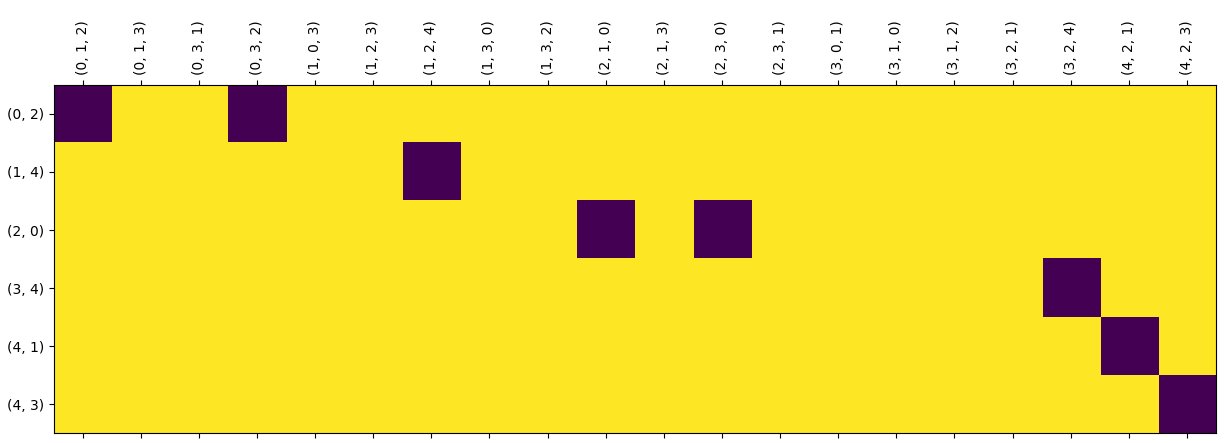
\includegraphics[scale=0.4]{images/kernel_toy_example_plain.png}
	%\caption{Matrix representation of $\partial_2:\widehat{M}_{2,2}(G) \to \widehat{M}_{1,2}(G)$. The $+1$ entries are represented in purple, while the $0$ entries are filled with yellow.}
	%\label{matrix_toyexample_normalized}
	%\end{figure}
	
	%\end{example}
	
	Let us now consider the other magnitude homology groups $\widehat{H}_k^{k-1}$ for $k>3$ and the corresponding differential matrices $\widehat{\Delta}_k^{k-1}$.
	By Definition~\ref{def:dif_matrix}, the null columns $\widehat{\Delta}_k^{k-1}$ correspond to $k$-trails $\overline{x}^k$ s.t. for any required vertex $x_i$ to be removed, $\len(\overline{x}^k_{\hat{\imath}})<k-1$. In particular, a null column corresponding to a generator $\overline{x}^k$ implies that there is an edge $\{x_{i-1},x_{i+1}\}~\forall 1<i<k$. 
	
	Intuitively, the presence of such generators is related to the presence of $k$-cliques in $G$.
	The following lemma formalizes this intuition and provides an upper bound on the number of $k$-cliques in $G$.
	
	\begin{lemma}\label{lem:k_cliques}
		Let $Z$ be the number of null columns of $\widehat{\Delta}_k^{k-1}$. The number of $k$-cliques in $G$ is upper bounded by $$\left\lfloor\frac{2Z}{k!}\right\rfloor.$$
	\end{lemma}
	\begin{proof}
		We claim that a set of $k$ vertices $x_1,\ldots,x_k$ is a $k$-clique if and only if all their representative permutations are generators of $\widehat{M}_k^{k-1}$ and they correspond to null columns of $\widehat{\Delta}_k^{k-1}$. Let us prove the two implications.
		\begin{description}
			\item[($\Rightarrow$)] Since $x_1,\ldots,x_k$ constitute a clique, there is an edge $\{x_i,x_j\}~\forall i,j\in[1,k]$, implying that any $k$-trail with $x_1,\ldots,x_k$ as required vertices (in any order) is of length $k-1$, and thus if it is a representative $k$-trail it is a generator of $\widehat{M}_k^{k-1}$. Again because there is an edge between any pair of such vertices, removing any required vertex from one of these generators leads to a $(k-1)$-trail of length $k-2$, thus by Definition~\ref{def:dif_matrix} they all correspond to null columns of $\widehat{\Delta}_k^{k-1}$.
			\item[($\Leftarrow$)] 
		\end{description}
	\end{proof}
	
	%While this does not provide any direct bound on the occurrences of particular subgraphs in $G$ (as all the triangles can be counted using $\widehat{\Delta}_3^2$ alone), intuitively the presence of such elements is related to the presence of cliques and chordless cycles in $G$. To this aim, we will inspect the normalized homology groups corresponding to entries on the second diagonal of the rank matrix.
	
	\subsection{Second diagonal} %: counting 4-cliques and 5,6-``quasi-cliques''.}

We are concerned in this section with the analysis of the information contained in the groups $\widehat{H}_{k}^{k}$.

While the question about a general interpretation for all magnitude homology groups $\widehat{H}_{k}^{k}$ on the second diagonal remains open, we were able to understand part of the information contained in $\widehat{H}_3^3$: specifically, in the null columns of $\Delta_3^3$.
%\begin{definition}
%   We call a \emph{quasi clique} a cycle containing all triangles.\giuliaB{@Giulia, ame sembra che contenere tutti i triangoli sia proprio una definizione alternativa di cricca...forse intendi solo alcuni specifici triangoli?}
%   \giuliaM{Giulia avevo proprio fatto un errore di concetto nel conto. Sto riscrivendo e ho aggiunto due lemmini. sono giusti, non so se sono sufficienti.}
%\end{definition}
We believe the third normalized magnitude homology group on the second diagonal provides us with information regarding the number of chordless $4$-cliques and $5$-cycles in the graph.

Consider the following chain
\begin{equation*}
	\begin{matrix}
		... &\to & \widehat{M}_4^3      &\to & \widehat{M}_3^3            &\to & \widehat{M}_2^3 &\to & 0. \\
		&    & \vin              &    & \vin                    &    & \vin         &    &    \\
		&    & (x_1,x_2,x_3,x_4) &    & (x_1,\hat{x},x_3,x_4) &    & (x_1,\hat{x},\hat{y},x_4). & &
	\end{matrix}
\end{equation*}

%and assume $x_4 \neq \hat{x}$.
We focus on the null columns of the differential matrix $\Delta_3^3$, that is on the basis elements $(x_1,\hat{x_2},x_3,x_4)$ such that $\Delta_3^3(x_1,\hat{x_2},x_3,x_4)=0$.
Notice that if $(x_1,\hat{x_2},x_3,x_4) \in \ker(\Delta_3^3)$ then one of the following is true: either $\len(x_1,\hat{x_2},\hat{x_3},x_4)=1$ or $\len(x_1,\hat{x_2},\hat{x_3},x_4)=2$.

\begin{observation}
	Call $L_1$ and $L_2$ the subsets of the basis of $\widehat{M}_3^3$ such that $\len(x_1,\hat{x_2},\hat{x_3},x_4)=1$ and $\len(x_1,\hat{x_2},\hat{x_3},x_4)=2$, respectively.
	Then $L_1$ and $L_2$ for a partition of the null columns of $\ker(\Delta_3^3)$ and, consequently, of $\widehat{H}_3^3$.
	Indeed,... 
\end{observation}

\begin{lemma} \label{lemma:4chordless_precise}
	The number of basis elements $(x_1,\hat{x_2},x_3,x_4)$ of $\widehat{M}_3^3$ such that the induced path $(x_1,x_3,x_4)$ is eulerian, $(x_1,x_3,x_4)$ is the image of $\Delta_4^3$ and $\len(x_1,\hat{x_2},\hat{x_3},x_4)=1$ is exactly the number of chordless $4$-cycles in the graph. 
\end{lemma}
\giuliaM{dire che bisogna dividere per 8 perchè per ogni quadrato (1,2,3,4) abbiamo 4 4-trails ((1,2,3,4), (2,3,4,1), (3,4,2,1), (4,3,2,1)) e ad ognuno togliano i due vertici intermedi uno alla volta per avere un elemento di $\widehat{M}_3^3$.}

\begin{proof}
	First notice that assuming $(x_1,x_3,x_4)$ eulerian while $\len(x_1,\hat{x_2},x_3,x_4)=3$, imply the absence of the edge $(x_1,x_3)$.
	Further, it is clear the $\len(x_1,\hat{x_2},\hat{x_3},x_4)=\len(x_1,x_4)=1$ implies the existence of the edge $(x_1,x_4)$, and thus $(x_2,x_2,x_3,x_4)$ is an induced $4$-cycle.
	
	Now, the image of $\Delta_4^3$ contains the elements $(x_1,\hat{x_2},x_3,x_4) \in \widehat{M}_3^3$ such that $\len(x_1,\hat{x_2},x_3,x_4)=\len(x_1,x_2,x_3,x_4)$.  
	In other words, trails that do not contain the triangle $(x_2,x_3,x_4)$, and in particular the edge $(x_2,x_4)$.
\end{proof}

\begin{lemma}
	The number of basis elements $(x_1,\hat{x_2},x_3,x_4)$ of $\widehat{M}_3^3$ such that the induced path $(x_1,x_3,x_4)$ is eulerian, $(x_1,x_3,x_4)$ is the image of $\Delta_4^3$ and $\len(x_1,\hat{x_2},\hat{x_3},x_4)=2$ is bounds from above the number of chordless $5$-cycles in the graph. 
\end{lemma}
\giuliaM{credo che andando a guardare i generatori si possa anche trovare il numero preciso di 5-cicli chordless}
\begin{proof}
	Proceeding similarly as in the proof of Lemma \ref{lemma:4chordless_precise}, we point out that the hypotheses of $(x_1,x_3,x_4)$ being eulerian and $\len(x_1,\hat{x_2},x_3,x_4)=3$, mean the absence of the edge $(x_1,x_3)$.
	Now, $\len(x_1,\hat{x_2},\hat{x_3},x_4)=\len(x_1,x_4)=2$ tells us that either the edge $(x_2,x_4)$ exists, or there is a different path of length $2$ from $x_1$ to $x_4$ involving a new vertex $x_5$.
	
	In addition, being $(x_1,\hat{x_2},x_3,x_4)$ in the image of $\Delta_4^3$ we know that the trail does not contain the triangle $(x_2,x_3,x_4)$, and in particular the edge $(x_2,x_4)$, so we are able to exclude the first case.
	
	In conclusion, we are left with a $5$-cycle $(x_1,x_2,x_3,x_4,x_5)$ which is surely missing diagonals $(x_1,x_3)$, $(x_1,x_4)$ and $(x_2,x_4)$. 
\end{proof}



%\begin{table}
%\centering
%\begin{tabular}{rr|rrrrrr}
%&&&&$k$&\\
%&&1&2&3&4&5\\ 
%\hline                                                               
%   & 0 &5\\
%   & 1 & &10\\                                          
%   & 2 & & &10\\                                          
%$l$& 3 & & &[$\len =1$, $\len =2$] &10\\                                          
%   & 4 & & &   &30 &10\\                                         
%   & 5 & & &   &   &50 \\           
%\end{tabular}
%\caption{Ranks of $\widehat{H}_k^{\ell}(G)$ computed using Python \cite{code2022magnitude}}
%\label{table:cliques}
%\end{table}


%We recall the definition of \emph{diagonal graph} introduced by Hepworth and Willerton in \cite{hepworth2015categorifying}.

%\begin{definition}
%A graph $G$ is called diagonal if $H_k^{\ell} = 0$ whenever $\ell \neq k-1$.
%\end{definition}

%The provided interpretation of $\widehat{H}_3^3$ suggest the following fact.

%\begin{lemma}
%If a graph $G$ is diagonal, then it is clique-free.
%\end{lemma}

%\begin{proof}
%Suppose G is diagonal, then $H_k^{\ell} = 0$ whenever $\ell \neq k-1$ and by Remark \ref{NMHsubgroup} $\widehat{H}_l^{\ell}=0$ if $\ell \neq k-1$. 
%In particular $\widehat{H}_3^3=0$, meaning the graph contains no $4$-clique, and therefore no bigger clique.\qed
%\end{proof}

\section{Relation with clustering coefficients}

In Graph Theory, a clustering coefficient is a structural feature that measures the degree to which nodes in a graph tend to cluster together.
In other words, it tells how connected a vertex’s neighbors are to one another.
There are two existing versions of this measure.
The \emph{global}, which was designed by Wasserman and Faust in \cite{wasserman1994social} to give an overall indication of the clustering in the network, and the \emph{local}, first defined by Watts and Strogatz in \cite{watts1998collective} to give an indication about the tendency to cluster near a specific node.

In this section we provide a way to compute both clustering coefficients of a graph $G=(V,E)$ via $\widehat{H}_3^2$, determining thus a close relation between these tools.


\subsection{Local clustering coefficient}

The local clustering coefficient $C_i$ of a node $x_i$ describes the likelihood that the neighbours of $x_i$ are also connected.
To compute $C_i$ we consider the neighborhood $N_i$ of $x_i$, where $N_i=\{x_j:(x_i,x_j)=e_{ij}\in E\}$ and compute the fraction of the number of links between the vertices within $N_i$ divided by the number of links that could possibly exist between them.
That is, we set
\[
C_i = \frac{2\{e_{jk}:x_j,x_k \in N_i \text{ and } e_{jk}\in E\}}{d_i(d_i -1)},
\]
where $d_i=|N_i|$ is the degree of the vertex $x_i$.

In other words, we are dividing the number of triangles $x_i$ is part of by the number of $2$-trails of length $2$ containing $x_i$.

Therefore, call $\widehat{M}_{3,i}^2$ the subgroup of $\widehat{M}_3^2$ such that $x_i$ is the middle vertex of any $2$-trail, so $\widehat{M}_{3,i}^2=\{(x,x_i,y): \len(x,x_i,y)=2\}$.
Then, by Section \ref{FirstDiagonal}, the number of triangles containing $x_i$ is precisely the number of null columns of $\ker(\Delta_3^2(\widehat{M}_{3,i}^2))$.
Calling this number $Z_i$, we can write the local clustering coefficient as
\[
C_i = \frac{2 Z_i}{d_i(d_i -1)}.
\]

\begin{remark}
	Given the connection just established between the local clustering coefficient and normalized magnitude homology, one could think of using $\widehat{H}_3^2$ in a network analysis context as a \emph{centrality measure}: if for a given vertex $v_i$ the number $Z_i$ defined above takes low values it means there are few connections between neighbors of $x_i$, meaning $x_i$ has a lot of power over information flow. 
\end{remark}


\subsection{Global clustering coefficient}

The global clustering coefficient $C$ is based on $3$-trails, i.e. on elements of $\widehat{M}_3^2$, and is computed as the number of closed $3$-trails (or $3  \times$ triangles) over the total number of $3$-trails (both open and closed).
That is, calling $Z$ the number of null columns in $\ker(\Delta_3^2(\widehat{M}_3^2))$
\[
C = \frac{Z}{|\widehat{M}_3^2|}. 
\]


\section{Algorithm complexity}

\section{Conclusions}

\appendix
\section{Formal Algebraic Definitions}\label{app:algebra}

\begin{definition}[\cite{hepworth2015categorifying}]\label{def:magchain}
	Consider the graph $G=(V,E)$.
	The $(k,\ell)$-magnitude chain $MC_{k,\ell}(G)$ is the free abelian group generated by the $k$-trails of length $\ell$ in $G$.
\end{definition}

\begin{definition}[\cite{hepworth2015categorifying}]
	\label{differential}
	Let $(x_0,\dots,\hat{x_i},\dots,x_k)$ denote the $k$-tuple obtained by removing the $i$-th vertex from the $(k+1)$-tuple $(x_0,\dots,x_k)$.  We define the differential 
	\[
	\partial_k: MC_{k,\ell}(G) \to MC_{k-1,\ell}(G)
	\]
	as the sum $\partial_k= \sum_{i=1}^{k-1} \partial_{k,i}$ of the maps defined by 
	\[
	\partial_{k,i}(x_0,\dots,x_k) = a_i\cdot(x_0,\dots,\hat{x_i},\dots,x_k),
	\]
	where
	\[a_i=\begin{cases}
		(-1)^{i+1} &\text{ if } \len(x_0,\dots,\hat{x_i},\dots,x_k) = \ell, \\
		0 &\text{ otherwise.}\\
	\end{cases}
	\]
\end{definition}

\begin{definition}[Magnitude chain complex]\label{def:magchaincomplex}
	We indicate as $M_{*,\ell}(G)$ the following sequence of free abelian groups connected by differentials
	\[
	\cdots \to M_{k+2,\ell}(G) \xrightarrow{\partial_{k+2}} M_{k+1}^{\ell} \xrightarrow{\partial_{k+1}} M_{k}^{\ell} \xrightarrow{\partial_{k}} M_{k-1}^{\ell} \to \cdots
	\]
\end{definition}

It is shown in \cite[Lemma 11]{hepworth2015categorifying} that the composition of two consecutive differentials $\partial_{k+1} \circ \partial_k$ vanishes, so that each chain $M_{*,\ell}(G)$ is indeed a chain complex (as for the standard definition given in \cite{hatcher2005algebraic}) and it is thus possible to define its $k$-th homology group.
%\giuliaM{Il fatto è che perché una sequenza di gruppi e mappe sia un complesso di catene è necessario che la composizione di due mappe consecutive si annulli, però non volevo appensantire con troppe defnizioni. Ho modificato un pochino il paragrafo, si capisce di più?}

\begin{definition}
	\label{def_MH}
	The $k$-magnitude homology group of the graph $G$ at level $\ell$ is the abelian group defined by
	\[
	MH_{k,l}(G) = H_k(M_{*,l}(G)) = \frac{\ker(\partial_k)}{\imm(\partial_{k+1})}.
	\]
\end{definition}


Contare colonne nulle è in P-space; elencarle no, perchè sono un numero esponenziale. Macchina di touring non det. può contare colonne nulle: il numero di combo accettate sono il numero di colonne nulle. 
Oracolo per problemi in $P^\{\# P\}\subseteq P$ space (problemi di conteggio su NDTM). Scriverli tutti richiede spazio esponenziale.

\bibliographystyle{plain}
\bibliography{bibliography.bib}


\end{document}